\documentclass[a4paper, 11pt]{article}
%\usepackage[T1]{fontenc}
\usepackage[utf8]{inputenc}
\usepackage[brazil]{babel}
\usepackage{graphicx}
\usepackage{listings}
\usepackage{amsmath}

\linespread{1.05}

\title{{\huge \bf Estudo de Técnicas para Geração Procedural de Arquitetura em um Ambiente 3D} \\ Relatório final de Iniciação}

\author{Felipe Santos Oliveira}

\begin{document}
    \pagenumbering{gobble}
    \maketitle
    \newpage
    
    \pagenumbering{roman}
    \tableofcontents
    \newpage
    \pagenumbering{arabic}

    \section{Introdução}
    Geração de conteúdo para mundos virtuais é uma área em constante crescimento, e usar artistas para a geração de cada \textit{asset} de uma cena é algo que pode sair bastante caro na produção de um jogo, filme ou aplicativo de realidade virtual. Com isso em mente, ao longo dos anos várias técnicas de geração de conteúdo de maneira procedural foram desenvolvidas, abrangindo a geração desde a história de um mundo à geração de planetas com biomas e climas beasados em modelos reais. 

    Um aspecto que recebe bastante atenção devido a suas diversas aplicações é a área de geração de arquitetura e cidades. As aplicações para a geração de conteúdo nesse setor vão desde a geração de cidades e ambientes urbanos em jogos a planejamento urbano de cidades reais, usando técnicas de \textit{crownd simulation} para simular o fluxo de indivíduos dentro de uma cidade e tomar decisões se baseando nos resultados das simulações. 

    Abordarei no estudo três técnicas principais: o uso de uma \textit{shape grammar} desenvolvida por \cite{Muller:2006:PMB:1141911.1141931}, o uso de L-Systems para a especifição de operações de \textit{morphing} em uma \textit{mesh} afim de gerar a geometria da arquitetura \cite{Parish:2001:PMC:383259.383292} e por fim um método híbrido de geração de arquitetura usando \textit{shape grammars} e operações de \textit{morphing} \cite{Zawadzki:2013:GSTF}.

    \section{\textit{L-Systems}} \label{sec:lsystem}
    \textit{L-System} é um tipo de gramática formal desenvolvido por A. Lindenmayer \cite{Prusinkiewicz:1996:ABP:235579} que consiste em um alfabeto de símbolos que podem ser usados para gerar cadeias de caracteres, uma coleção de regras de produção que expande cada símbolo, um axioma inicial de onde se inicia a construção e um mecanismo para traduzir as cadeias formadas em geometria. Formalmente,

    $$ L_S = (V, \omega, P) $$

    onde $V$ é o alfabeto de símbolos, $\omega$ o axioma de início e $P$ a coleção de regras de produção. 

    \begin{center}
        \begin{lstlisting}[language=sh,caption=Triângulo de Sierpinski, frame=single, basicstyle=\ttfamily\small, captionpos=b]
alphabet: A B
constants: + -
axiom: A
rules: (A -> +B-A-B+), (B -> -A+B+A-)
angle: 60
        \end{lstlisting}
        \label{lst:sierpinski}
    \end{center}

    \begin{figure}[h]
        \centering
        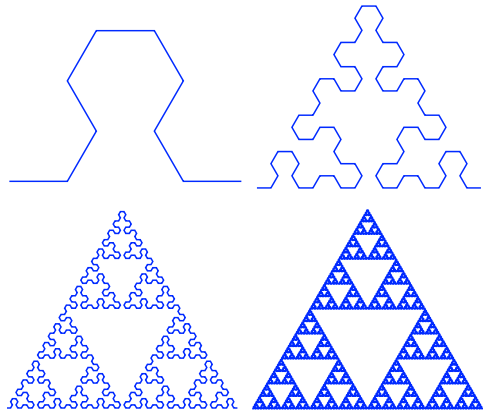
\includegraphics[width=\textwidth]{imgs/sierpinski.png}
        \caption{Triângulo de Sierpinski gerado por \textit{L-System}}
        \label{fig:sierpinski}
    \end{figure}

    \textit{L-systems} podem ser expandidos de forma a torná-los paramétricos, isto é, cada símbolo tem associado a si um conjunto de parâmetros usados para modificar características específicas daquele símbolo, e estocásticos, associando uma probabilidade a regras de produção. 

    Usando esses conceitos, \cite{Parish:2001:PMC:383259.383292} desenvolveu um \textit{L-system} estocático e paramétrico que executa transformações geométricas e operações de extrusão, ramificação e terminação. O axioma usado é a \textit{bounding box} do lote do prédio e a forma final da estrutura se dá pela interpretação da saída do \textit{L-system}.

    \begin{figure}[h]
        \centering
        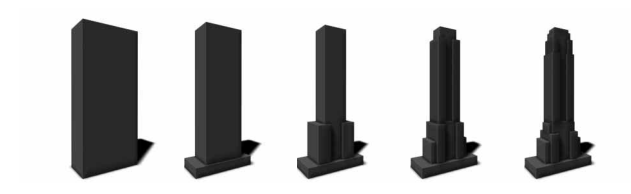
\includegraphics[width=\textwidth]{imgs/skyscrapper.png}
        \caption{Arranha-céu gerado após 5 iterações do algorítimo.}
        \label{fig:skyscrapper}
    \end{figure}    

    O método descrito considera três tipos de prédios na hora da geração: arranha-céus, prédios comerciais e casas residênciais, e o tipo de prédio a ser gerado é baseado na zona onde o lote se encontra, assim como outras restrições como prédios vizinhos e altura máxima. Apesar de poder gerar uma grande variedade de estruturas, o método descrito tem a limitação de ter que usar regras complexas em sua geração. 
        
    \section{\textit{Shape Grammars}} \label{sec:shape}
    \textit{Shape grammars} são gramáticas que especificam regras de produção para geração de formas geometricas em 2D ou 3D. Formalmente, uma \textit{shape grammar} pode ser descrita como uma tupla \cite{Zawadzki:2013:GSTF}

    $$ S_G := <V_T, V_M, R, A> $$  

    onde $S_G$ é a gramática, $V_T$ é um conjunto de formas terminais, $V_M$ um conjunto de formas não-terminais, $R$ um conjunto finito de regras de produção e $A$ o axioma de início. A ideia de \textit{shape grammars} é algo que vem da arquitetura, criada em 1971 por \cite{Stiny71shapegrammars} com o objetivo de servir de ferramenta no design de prédios e arte. 

    Em \cite{Muller:2006:PMB:1141911.1141931}, os autores descrevem uma \textit{shape grammar} baseada nas ideias dos \textit{L-systems} \ref{sec:lsystem} em questão de notação e implementação. A gramática funciona com uma configuração de formas que possuem atributos como posição e tamanho, um símbolo único e uma geometria. A posição o tamanho definem uma \textit{bounding box} que serve de escopo para a manipulação da geometria da forma.

    O processo de produção é uma configuração de um conjunto finito de formas, e pode comecar de uma forma arbitrária $A$, o axioma, e segue da seguinte forma:

    \begin{enumerate}
        \item Selecione uma forma ativa com símbolo $B$ no conjunto
        \item Escolha uma regra de produção com $B$ no \textit{lhs} para computar um sucessor de $B$, $B_{NEW}$
        \item Marque $B$ como inativo e adicione $B_{NEW}$ à configuração, e volte ao passo 1
    \end{enumerate}

    A produção cessa quando não há mais nenhum símbolo não terminal na configuração. Ao final temos uma árvore de derivação que pode ser percorrida em \textit{BFS} com o uso de uma prioridade para regras mais importantes. 

    Regras de produção possuem a seguinte notação:

    $$A \rightarrow \text{function}(\text{parameters})\{\text{children}\}:\text{probability}$$

    As principais regras são: 

    \begin{itemize}
        \item \textbf{Escopo}: regras para transformação de formas, como translação, escalamento e rotação. É usada diretamente em formas geométricas pré-definidas, como cubos, cilindros e pirâmides, além de definir qual o escopo atual para outras operações. Abaixo pode-se ver um exemplo onde colocamos um cubo na área de produção:

        $$A \rightarrow T(0,0,6) S(8,10,8) I(\text{``cube''})$$

        onde $T$ é a operação de translação, $S$ a de escala e $I$ a função que chama o escopo sobre o cubo.

        \item \textbf{Divisão}: divide o escopo atual em função de um eixo. Por exemplo:

        $$A \rightarrow subDiv("Y",3.5,0.3,3,3,3)\{floor|ledge|floor|floor|floor\}$$

        Temos que a divisão, neste caso, se dá no eixo $Y$, e os valores em parâmetros definem os tamanhos das divisões. Os elementos dentro das chaves definem os símbolos associados a cada parte da divisão, que serão posteriormente trabalhados por regras próprias. A regra se aplica a múltiplos eixos, como por exemplo $XY$ ou $XYZ$.

        \item \textbf{Dimensionamento}: às vezes queremos usar um valor de referência em uma regra, como uma fração do valor de um eixo do tamanho do escopo ou uma proporção entre as partes. Para isso usamos uma notação de referenciamento de valores, onde podemos referenciar valores do escopo ou passar valores absolutos.

        \item \textbf{Repetir}: permite a repetição de estruturas grandes e complexas.

        $$A \rightarrow repeat("X",2)\{B\}$$

        Podemos escolher repetir somente um eixo de modo a criar um espelhamento ou a estrutura toda, passando também o número de repetições que queremos fazer.

        \item \textbf{Divisão em componentes}: permite a divisão de um escopo em elementos de menor dimensão, como faces ou vertices de uma face.

        $$a \rightarrow comp(type, param)\{A|B|C...\}$$
    \end{itemize}

    Com o uso destas regras, se é possível gerar formas tri-dimensionais complexas, mas não sem seus problemas. Quanto mais complexa a forma, mais o uso de simples operações como a união faz com que polígonos complexos apareçam nas cascas das estruturas, como buracos, polígonos concavos e uma quantidade grande vértices. 

    Para contornar essas situações, a gramática permite a geração de estruturas bidimensionais através da divisão em componentes, gerandos escopos 2D. Estes escopos estarão correntamente alinhados e parametrizados com as fachadas e telhados após a extração das componentes. Por fim, a gramática pode prosseguir refinando os triângulos e quads resultantes. 

    \begin{center}
        \begin{lstlisting}[language=sh,caption=Exemplo de \textit{Shape Grammar}, frame=single, basicstyle=\ttfamily\small, captionpos=b]
lot -> S(1r,building height,1r)
       Subdiv("Z",Scope.sz*rand(0.3,0.5),1r)
                { facades | sidewings }
sidewings -> Subdiv("X",Scope.sx*rand(0.2,0.6),1r)
                { sidewing | e }
             Subdiv("X",1r,Scope.sx*rand(0.2,0.6))
                { e | sidewing }
sidewing
         -> S(1r,1r,Scope.sz*rand(0.4,1.0)) facades : 0.5
         -> S(1r,Scope.sy*rand(0.2,0.9),
                Scope.sz*rand(0.4,1.0))facades : 0.3
         -> e : 0.2
facades -> Comp("sidefaces"){ facade }
        \end{lstlisting}
        \label{lst:shapegrammar}
    \end{center}

    \begin{figure}[h]
        \centering
        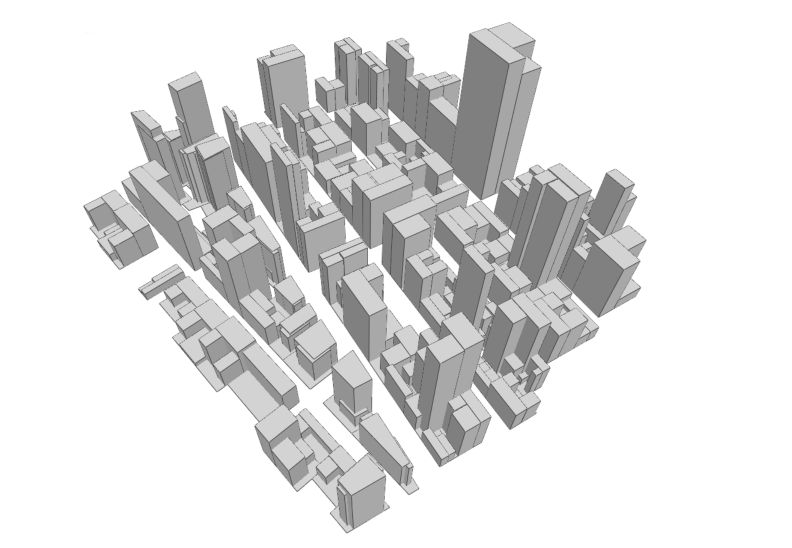
\includegraphics[width=\textwidth]{imgs/grammarcity.png}
        \caption{Vizinhança gerada pela gramática acima.}
        \label{fig:skyscrapper}
    \end{figure}  

    \section{Método Híbrido} \label{sec:hybrid}
    O método híbrido descrito por \cite{Zawadzki:2013:GSTF} consite no uso de \textit{shape grammars} junto de operações de metamorfose nas \textit{meshes}. Metamorfose (ou \textit{morphing}) nesse contexto pode ser definido como um processo contínuo e suave de transformação de uma forma em outra, e pode ser divido em um problema de dois passos: o primeiro é que, dada uma forma, devemos determinar quais as características da forma devem ser transformadas e a interpolação de formas de acordo com certas trajetórias; o segundo é o resultado da primeiro, uma forma intermediária que pode conter características topológicas de ambas formas usadas na transformação. Esta forma intermediária o ator principal desse método.

    O método híbrido combina o conceito das \textit{shape grammars} de usar uma representação hierárquica de formas, junto de um conjunto de operações (ou regras) e da metamorfose contínua de formas na forma de uma regra extra, em adição às regras discretas da gramática.

    Regras de formas, em geral, possuem operações booleanas como soma, diferença e união. Chamamos essas regras de regras clássicas ($R_C$). A regra mórfica chamamos de $R_M$, que funciona transformando duas formas de entrada em uma forma de saída usando um parâmetro de interpolação linear.

    \begin{figure}[h]
        \centering
        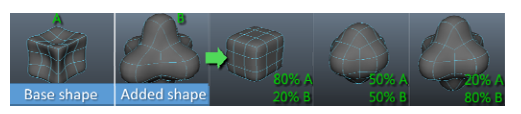
\includegraphics[width=\textwidth]{imgs/morph.png}
        \caption{Aplicação de uma regra de adição em $R_M$.}
        \label{fig:morph}
    \end{figure}  

    \begin{figure}[!ht]
        \centering
        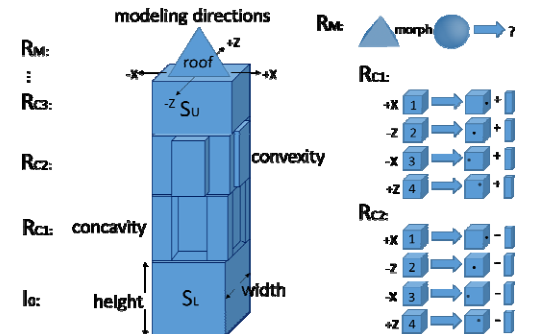
\includegraphics[width=60mm]{imgs/hybridbuilding.png}
        \caption{Geração de um prédio pelo método híbrido.}
        \label{fig:hybridblock}
    \end{figure}      

    Para a geração de arquitetura, o método faz a suposição de que o prédio terá vários andares. A partir daí, inicia-se com uma regra para o térreo e com a regra para o último andar, e as regras podem ser criadas usando interpolação linear. Para cada nível, determinamos características como altura, largura e convexidade. Após a aplicação da última regra, podemos modelar o telhado mergindo uma forma afiada (uma pirâmide) a uma forma esférica. 

    \begin{figure}[!ht]
        \centering
        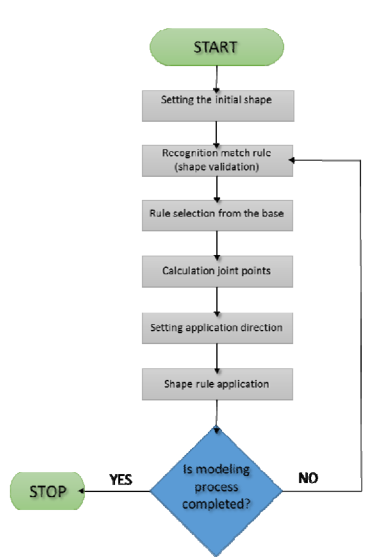
\includegraphics[width=60mm]{imgs/hybridblock.png}
        \caption{Bloco principal do algorítimo híbrido.}
        \label{fig:hybridblock}
    \end{figure}    

    \section{Implementação} \label{sec:impl}
    Dentre os métodos abordados, realizei a implementação de \cite{Muller:2006:PMB:1141911.1141931}. A implementação foi realizada em Python e OpenGL, e consistiu de um parser para o arquivo de regras, um construtor da árvore de derivação e o construtor da geometria com base na árvore.

        \subsection{Parser}
        Regras são compostas de símbolos, funções e parâmetros. O objetivo do parser é quebrar o conjunto de regras em pedaços lógicos que possam ser trabalhados pelas etapas seguintes da pipeline, já gerando uma árvore hierárquica que vai servir de base para a geração da árvore de modelos.

        \subsection{Construtor de Árvore de Modelos}
        A árvore de modelos ou árvore de derivação contém as primitivas geométricas que vão dar origem à \textit{mesh} ao final da pipeline. É nessa etapa que percorremos a árvore de regras e executamos as funções citadas no artigo.

        Devido ao escopo do projeto, me limitei a implementar somente as operações básicas, como translação, escalamento, divisão simples, divisão por componentes e repetição. 

        \begin{center}
        \begin{lstlisting}[language=python,caption=Laço principal do contrutor da árvore de derivação., frame=single, basicstyle=\ttfamily\small, captionpos=b]
while not self.queue.empty():
    currentShape = self.queue.get();

    if currentShape.id in ruleset:
        rules = ruleset[currentShape.id]

        if len(rules) <= 1:
            index = 0

        function = rules[index].name

        if function == "comp":
            self.comp(rules[index].childName, 
              currentShape)
        elif function == "S":
            self.s(rules[index].parameters, 
              rules[index].childName, currentShape)
        elif function == "T":
            self.t(rules[index].parameters, 
              rules[index].childName, currentShape)
        elif function == "repeat":
            self.repeat(rules[index].parameters, 
              rules[index].childName, currentShape)
        elif function == "subDiv":
            self.subDiv(rules[index].parameters, 
              rules[index].childName, currentShape)
        else:
            self.null(rules[index].childName, 
              currentShape)

    index = fixedIndex
        \end{lstlisting}
        \label{lst:derivation}
    \end{center}

    A função \texttt{null} neste caso significa uma regra terminal, dado que ela não gera uma lista de filhos.

        \subsection{Construtor de Geometria}
        Por fim, uma vez que possuimos a árvore de derivação com todos seus componentes e posições, podemos realizar a geração da geometria do prédio. Para simplificar o processo, temos somente três simbolos terminais: paredes, portas e janelas. 

        Uma vez que encontramos um objeto que pertença a uma dessas classificações, o marcamos utilizando coordenadas de textura, que serão passadas para um shader, onde iremos destacar, em tons de cinza, cada parte da \textit{mesh} final. Fazemos também o cálculo de normais para a iluminação difusa da cena.

    \section{Resultados} \label{sec:res}
    Montando um conjunto de regras, realizei um experimento para a geração de um prédio simples. O conjunto de regras utilizado pode ser visto no \ref{sec:apendix}. Os resultados podem ser vistos abaixo:

    \begin{figure}[h]
        \centering
        
\includegraphics[width=45mm]{imgs/building1.png} 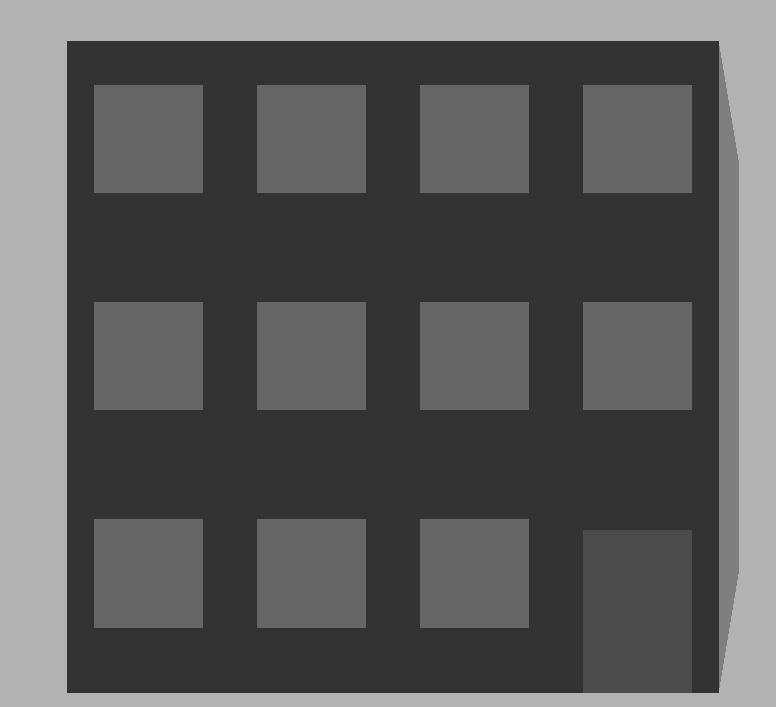
\includegraphics[width=45mm]{imgs/building2.png}
        \caption{Prédios construidos a partir do mesmo conjunto de regras.}
        \label{fig:testbuilding}
    \end{figure}

    Os prédios gerados são provenientes do mesmo conjunto de regras, mostrando o aspecto estocástico da gramática implementada.

    \section{Conclusão e Considerações Finais} \label{sec:con}
    Através desse estudo pudemos ver diferentes métodos de geração de arquitetura de modo procedural. Dentre os vistos, o mais simples e efetivo parece ser o método que usa \textit{shape grammar}, dado que a estrutura da gramática e as regras de produção são de certo modo intuitivas e fáceis de entender. O método que usa \textit{L-systems} se mostra efetivo quando se está trabalhando em cima de uma forma básica, como um cubo, cilindro e pirâmides, pois a gramática permite transformações geométricas diversas de maneira direta, diferente do visto com as \textit{shape grammar}, onde transformações como uniões, somas e diferenças não são claras de se ver. Por fim, o último método abordado, o método híbrido, apesar de sere interessante pelo paradigma de usar metamorfose de formas, se mostra complexo comparado com os outros, e parece ser menos abrangente devido às suposições feitos pelo autor.

    Vale lembrar que existem inúmeros outros métodos que não foram abordados nesse estudo, como uso de fractais, diagramas de Voronoi para demarcação de lotes, combinação de primitivas geométricas através da superposição de formas geométricas bidimensionais, entre outros. Em estudos futuros esses métodos serão abordados e o estudo como um todo servirá de base para a posterior criação de um novo método de geração de arquitetura com o uso de gramáticas.

    
    \newpage
    
    \bibliographystyle{abbrv}
    \bibliography{references}

    \section{Apêndice} \label{sec:apendix}
        \subsection{Conjunto de regras usado no teste}
        \begin{center}
        \begin{lstlisting}[language=sh,caption=Conjunto de regras, frame=single, basicstyle=\ttfamily\small, captionpos=b]
start -> S(12,12,12){lot}
lot -> comp(){top|left_facade|front|
              right_facade|back|bottom}
back -> wall

front -> subDiv("Y",6,6){gfloor|ffloor}:0.6
front -> subDiv("Y",4,4,4){gfloor|ffloor|ffloor}:0.4
left_facade -> subDiv("Y",6,6){lfloor|lfloor}:0.6
left_facade -> subDiv("Y",4,4,4){lfloor|
                                 lfloor|lfloor}:0.4

right_facade -> subDiv("Y",6,6){rfloor|rfloor}:0.6
right_facade -> subDiv("Y",4,4,4){rfloor|
                                  rfloor|rfloor}:0.4

gfloor -> subDiv("X",9,3){ftiles|entrance}:0.6
gfloor -> subDiv("X",3,9){entrance|ftiles}:0.4
ffloor -> ftiles
ftiles -> repeat("X",3){ftile}

lfloor -> ltiles
ltiles -> repeat("Z",3){ltile}

rfloor -> rtiles
rtiles -> repeat("Z",3){rtile}


ftile  -> subDiv("X",0.5,2,0.5){fwall|
                            fwindow_area|fwall}
ltile  -> subDiv("Z",0.5,2,0.5){lwall|
                            lwindow_area|lwall}
rtile  -> subDiv("Z",0.5,2,0.5){rwall|
                            rwindow_area|rwall}

fwindow_area -> subDiv("Y",1.2,4,0.8)
                        {fwall|fwindow|fwall}:0.6
fwindow_area -> subDiv("Y",1.2,2,0.8)
                        {fwall|fwindow|fwall}:0.4

lwindow_area -> subDiv("Y",1.2,4,0.8)
                        {lwall|lwindow|lwall}:0.6
lwindow_area -> subDiv("Y",1.2,2,0.8)
                        {lwall|lwindow|lwall}:0.4

rwindow_area -> subDiv("Y",1.2,4,0.8)
                        {rwall|rwindow|rwall}:0.6
rwindow_area -> subDiv("Y",1.2,2,0.8)
                        {rwall|rwindow|rwall}:0.4

fwindow -> window
lwindow -> window
rwindow -> window

fwall -> wall
lwall -> wall
rwall -> wall

entrance -> subDiv("X",0.5,2,0.5){wall|door_area|wall}
door_area -> subDiv("Y",5,1){door|wall} :0.6
door_area -> subDiv("Y",3,1){door|wall} :0.4
        \end{lstlisting}
        \label{lst:testrules}
    \end{center}
\end{document}
